
% part 5
\section{Улучшенная Twisted поэзия\label{sec:part5}}


\subsection{Абстрактный экспрессионизм}

%In Part 4 we made our first poetry client that uses Twisted. It works pretty well, but there is definitely room for improvement.

В предыдущей главе мы сделали наш первый поэтический клиент, 
использующий Twisted. Он работает достаточно хорошо, но в нем определенно 
есть что улучшить.


%First of all, the client includes code for mundane details like creating network sockets and receiving data from those sockets. Twisted provides support for these sorts of things so we don’t have to implement them ourselves every time we write a new program. This is especially helpful because asynchronous I/O requires a few tricky bits involving exception handling as you can see in the client code. And there are even more tricky bits if you want your code to work on multiple platforms. If you have a free afternoon, search the Twisted sources for “win32″ to see how many corner cases that platform introduces.


В первую очередь, клиент влючает код с такими деталями, 
как создание сетевых сокетов, получение данных из 
сокетов. Twisted поддерживает эти вещи, так что нам не нужно 
реализовывать их самим каждый раз, когда мы пишем новую программу. 
Это особенно удобно, поскольку асинхронный ввод-вывод 
требует нескольких хитростей, включающих обработку исключений, так как это 
делается в 
\href{http://github.com/jdavisp3/twisted-intro/blob/master/twisted-client-1/get-poetry.py}{коде клиента}. 
И есть много всяких хитростей, для того, чтобы сделать код 
работающим на нескольких платформах. Если у вас есть свободное 
время - поищите в исходниках Twisted слово "win32", для того, чтобы 
увидеть как много всяких проблем исходит от этой платформы.


%Another problem with the current client is error handling. Try running version 1.0 of the Twisted client and tell it to download from a port with no server. It just crashes. We could fix the current client, but error handling is easier with the Twisted APIs we’ll be using today.


Другая проблема в текущем клиенте - обработка ошибок. Попробуйте 
запустить версию 1.0 Twisted клиента и укажите порт, на котором 
не запущен сервер. Программа просто разрушится. Мы могли бы 
исправить текущий клиент, но управление ошибками проще делать 
с помощью Twisted API, которые мы сегодня будем использовать. 

%Finally, the client isn’t particularly re-usable. How would another module get a poem with our client? How would the “calling” module know when the poem had finished downloading? We can’t write a function that simply returns the text of the poem as that would require blocking until the entire poem is read. This is a real problem but we’re not going to fix it today — we’ll save that for future Parts.

И наконец, клиент не является переиспользуемым. Как другой 
модуль мог бы получить поэму с помощью нашего клиента? Как  
"вызывающий" модуль узнал бы, когда поэма скачалась? Мы не можем 
написать функцию, которая просто возвращает текст поэмы, так как 
это потребовало бы блокирования до тех пор, пока вся поэма не 
прочитана. Это реальная проблема, но мы не собираемся исправлять 
ее сегодня - мы это сделаем в следующих главах.


%We’re going to fix the first and second problems using a higher-level set of APIs and Interfaces. The Twisted framework is loosely composed of layers of abstractions and learning Twisted means learning what those layers provide, i.e, what APIs, Interfaces, and implementations are available for use in each one. Since this is an introduction we’re not going to study each abstraction in complete detail or do an exhaustive survey of every abstraction that Twisted offers. We’re just going to look at the most important pieces to get a better feel for how Twisted is put together. Once you become familiar with the overall style of Twisted’s architecture, learning new parts on your own will be much easier.

Мы собираемся исправить первую и вторую проблемы, используя 
высокоуровневое множество API и Interface'ов.

%In general, each Twisted abstraction is concerned with one particular concept. For example, the 1.0 client from Part 4 uses IReadDescriptor, the abstraction of a “file descriptor you can read bytes from”. A Twisted abstraction is usually defined by an Interface specifying how an object embodying that abstraction should behave. The most important thing to keep in mind when learning a new Twisted abstraction is this:

В целом, каждая Twisted абстрация касается только 
одной определенной концепции. Например, клиент 1.0 из 
главы 4 использует IReadDescriptor: абстракция 
"файлового дескритора, из которого можно прочитать данные". 
Twisted абстракция обычно определяется Interface'ом, 
задающим то, как объекту, воплощающему абстракцию, 
следует себя вести. Наиболее важная деталь, про которую надо 
помнить, следующая:

%Most higher-level abstractions in Twisted are built by using lower-level ones, not by replacing them.
Большинство высокоуровневых абстракций в Twisted построены 
с использованием низкоуровневых, не заменяя их.


%So when you are learning a new Twisted abstraction, keep in mind both what it does and what it does not do. In particular, if some earlier abstraction A implements feature F, then F is probably not implemented by any other abstraction. Rather, if another abstraction B needs feature F, it will use A rather than implement F itself.  (In general, an implementation of B will either sub-class an implementation of A or refer to another object that implements A).

Поэтому, когда вы изучаете новую Twisted абстракцию, 
поймите, что она делает и что не делает. Особенно, если 
некоторая более ранняя абстракция A реализует свойство F, 
то F вероятно не реализована другой абстракцией. 
Пожалуй, если другой абстракции B нужно свойство F, 
она будет переиспользовать А нежели, чем реализовывать F 
сама (реализация B будет либо наследовать реализацию 
A, либо ссылаться на другой объект, который реализует A). 

%Networking is a complex subject, and thus Twisted contains lots of abstractions. By starting with lower levels first, we are hopefully getting a clearer picture of how they all get put together in a working Twisted program.

Сети - сложный предмет, так что Twisted содержит множество 
абстракций. Начиная с низкого уровня, мы получим 
более ясную картину того, как все соединяется вместе в 
работающей Twisted программе.


\subsection{Без цикла в мозге}

%The most important abstraction we have learned so far, indeed the most important abstraction in Twisted, is the reactor. At the center of every program built with Twisted, no matter how many layers that program might have, there is a reactor loop spinning around and making the whole thing go. Nothing else in Twisted provides the functionality the reactor offers. Much of the rest of Twisted, in fact, can be thought of as “stuff that makes it easier to do X using the reactor” where X might be “serve a web page” or “make a database query” or some other specific feature. Although it’s possible to stick with the lower-level APIs, like the client 1.0 does, we have to implement more things ourselves if we do. Moving to higher-level abstractions generally means writing less code (and letting Twisted handle the platform-dependent corner cases).

Наиболее важная абстракция, которую мы узучили до сего 
момента, являющаяся самой важной абстракцией в Twisted, - 
reactor. В центре каждой программы, построенной с 
помощью Twisted, невзирая на количество уровней, которые 
программа может иметь, существует реакторный цикл, в 
котором осуществляются все запуски. В Twisted функциональность 
реактора реализована только в реакторе. Об остальном в Twisted 
можно думать как о "вещах, упрощающих реализацию X, использующего reactor", 
где X - может быть "обслужить web страницу" или "сделать запрос к базе", 
или что-то подобное. Хотя можно придерживаться низкоуровневых API, 
подобных тому, что делает клиент 1.0, но в этом случае мы должны реализовать 
больше всяких мелочей. Перемещение на более высокий уровень 
абстракций в основном означает, что кода будет меньше (и позволяет 
Twisted управлять зависимыми от платформы ньюансами).


%But when we’re working at the outer layers of Twisted it can be easy to forget the reactor is there. In any Twisted program of reasonable size, relatively few parts of our code will actually use the reactor APIs directly. The same is true for some of the other low-level abstractions. The file descriptor abstractions we used in client 1.0 are so thoroughly subsumed by higher-level concepts that they basically disappear in real Twisted programs (they are still used on the inside, we just don’t see them as such).

Но, когда мы работаем на внешних уровнях Twisted, 
можно просто забыть про reactor. В Twisted 
программе разумного размера, относительно мало 
частей кода будут действительно использовать 
API реактора напрямую. Тоже самое верно для других 
низкоуровневых абстракций. Абстракции файлового 
дескриптора, которые мы использовали в клиенте 1.0, 
являются также тщательно включенными высокоуровневыми 
концепциями, они в основном не видны в реальных 
Twisted программах (они все еще используются внутри, 
но мы их просто не видим как таковых).


%As far as the file descriptor abstractions go, that’s not really a problem. Letting Twisted handle the mechanics of asynchronous I/O frees us to concentrate on whatever problem we are trying to solve. But the reactor is different. It never really disappears. When you choose to use Twisted you are also choosing to use the Reactor Pattern, and that means programming in the “reactive style” using callbacks and cooperative multi-tasking. If you want to use Twisted correctly, you have to keep the reactor’s existence (and the way it works) in mind. We’ll have more to say about this in Part 6, but for now our message is this:

Поскольку абстракции файловых дескрипторов работают, 
то можно позволить Twisted 
управлять механизмами асинхронного ввода-вывода и освободить  
нас для концентрации над тем, что мы действительно хотим 
решить. Но reactor отличается. Он в действительности никогда 
не исчезнет. Когда вы выбираете использование Twisted, 
вы также выбираете использование шаблона проектирования Reactor, 
и это означает программированкооперативнойном стиле", 
с использованием callback'ов и кооперативной многозадачности 
(cooperative multi-tasking). Если вы хотите использовать 
Twisted корректно, вы должны помнить про существование реактора  и 
про то, как он работает. В главе 6 будет больше сказано про это, резюмируя 
можно сказать:

%Figure 5 and Figure 6 are the most important diagrams in this introduction.
Рисунки \ref{fig:reactor-1} и \ref{fig:reactor-callback} - самые 
важные в данном введении. 


%We’ll keep using diagrams to illustrate new concepts, but those two Figures are the ones that you need to burn into your brain, so to speak. Those are the pictures I constantly have in mind while writing programs with Twisted.
Мы будет иллюстрировать новые концепции, но эти 
два рисунка обязательно нужно запомнить и держать в голове 
при написании программ с использованием Twisted.

%Before we dive into the code, there are three new abstractions to introduce: Transports, Protocols, and Protocol Factories.
До того, как мы погрузимся в код, нужно ознакомиться с тремя 
новыми абстракциями: Transport, Protocol и Protocol Factory.


\subsection{Транспорты}

%The Transport abstraction is defined by ITransport in the main Twisted interfaces module. A Twisted Transport represents a single connection that can send and/or receive bytes. For our poetry clients, the Transports are abstracting TCP connections like the ones we have been making ourselves in earlier versions. But Twisted also supports I/O over UNIX Pipes and UDP sockets among other things. The Transport abstraction represents any such connection and handles the details of asynchronous I/O for whatever sort of connection it represents.

Абстракция Transport определяется в 
\href{http://twistedmatrix.com/trac/browser/tags/releases/twisted-8.2.0/twisted/internet/interfaces.py#L1289}{ITransport} 
в модуле Twisted \href{http://twistedmatrix.com/trac/browser/tags/releases/twisted-8.2.0/twisted/internet/interfaces.py}{interfaces}. Twisted Transport представляет одно соединение, которое 
может отправлять и/или получать байты. Для наших поэтических клиентов, 
Transport'ы - абстрактные TCP соединения подобно тем, которые мы делали в 
ранних версиях. Twisted также поддерживает ввод-вывод через 
\href{http://en.wikipedia.org/wiki/Unix\_pipe#Network\_pipes}{Unix pipe's} 
и UDP сокеты. Абстракция Transport предствляет любое такое 
соединение и управляет деталями асинхронного ввода-вывода для 
любого типа соединения, которое оно представляет.


%If you scan the methods defined for ITransport, you won’t find any for receiving data. That’s because Transports always handle the low-level details of reading data asynchronously from their connections, and give the data to us via callbacks. Along similar lines, the write-related methods of Transport objects may choose not to write the data immediately to avoid blocking. Telling a Transport to write some data means “send this data as soon as you can do so,  subject to the requirement to avoid blocking”. The data will be written in the order we provide it, of course.

Если посмотреть на методы, определенные для ITransport, 
то там ничего не будет про получение данных. Поскольку 
Transport'ы всегда управляют низкоуровневыми деталями 
асинхронного чтения данных из их соединений, 
и дают нам данные через callback'и. Среди подобных строк, 
методы объектов типа Transport, имеющие отношение к записи, 
могут не записывать данные тут же, избегая блокирования. 
Говоря Transport'у записать некоторые данные означает 
"отправьте эти данные так скоро, как вы сможете это 
сделать, избегая блокирования". Данные будут записаны, конечно же, 
в том же порядке, в котором мы их предоставили.   

%We generally don’t implement our own Transport objects or create them in our code. Rather, we use the implementations that Twisted already provides and which are created for us when we tell the reactor to make a connection.

В общем мы не реализовываем свой свои собственные Transport 
объекты или не создаем их в нашем коде. Скорее, мы используем 
реализации, которые Twisted уже предоставил и которые создаются 
для нас, когда мы говорим реактору сделать соединение.   


\subsection{Протоколы}

%Twisted Protocols are defined by IProtocol in the same interfaces module. As you might expect, Protocol objects implement protocols. That is to say, a particular implementation of a Twisted Protocol should implement one specific networking protocol, like FTP or IMAP or some nameless protocol we invent for our own purposes. Our poetry protocol, such as it is, simply sends all the bytes of the poem as soon as a connection is established, while the close of the connection signifies the end of the poem.

Twisted Protocol'ы определены в
\href{http://twistedmatrix.com/trac/browser/tags/releases/twisted-8.2.0/twisted/internet/interfaces.py#L1111}{IProtocol} 
в том же модуле 
\href{http://twistedmatrix.com/trac/browser/tags/releases/twisted-8.2.0/twisted/internet/interfaces.py}{interfaces}. 
Как Вы могли бы ожидать, объекты типа Protocol реализуют  
\href{http://en.wikipedia.org/wiki/Protocol\_(computing)}{протоколы}. 
Нужно сказать, что определеный Twisted Protocol реализует 
один определенный сетевой протокол, такой как 
\href{http://en.wikipedia.org/wiki/File\_Transfer\_Protocol}{FTP} или 
\href{http://en.wikipedia.org/wiki/Internet\_Message\_Access\_Protocol}{IMAP}, 
или какой-нибудь безымяный протокол, который мы изобрели 
для наших целей. Наш поэтический протокол, так как он есть, 
просто отправляет все байты поэмы в момент установления соединения до 
момента соединения, означающего конец поэмы. 

%Strictly speaking, each instance of a Twisted Protocol object implements a protocol for one specific connection. So each connection our program makes (or, in the case of servers, accepts) will require one instance of a Protocol. This makes Protocol instances the natural place to store both the state of “stateful” protocols and the accumulated data of partially received messages (since we receive the bytes in arbitrary-sized chunks with asynchronous I/O).

Строго говоря, каждый экземпляр объекта типа Twisted Protocol 
реализует протокол для одного определенного соединения. Поэтому 
каждое соединение, которое делает наша программа (или, в случае серверов, принимает), 
будет требовать один экземпляр Protocol. Это делает 
экземпляры типа Protocol естественным местом для хранения состояния 
протоколов и собранных данных из частично полученных сообщений (поскольку 
мы получаем куски произвольного размера, используя асинхронный ввод-вывод). 


%So how do Protocol instances know what connection they are responsible for? If you look at the IProtocol definition, you will find a method called makeConnection. This method is a callback and Twisted code calls it with a Transport instance as the only argument. The Transport is the connection the Protocol is going to use.

Так как же экземпляры Protocol узнают за какое соединение 
они ответственны? Если вы посмотрите на определение IProtocol, 
вы обнаружите метод с названием makeConnection. Этот метод - callback, и 
Twisted код вызывает его с экземпляром типа Transport в качестве 
единственного аргумента. Transport - соединение, которое Protocol 
будет использовать.

%Twisted includes a large number of ready-built Protocol implementations for various common protocols. You can find a few simpler ones in twisted.protocols.basic. It’s a good idea to check the Twisted sources before you write a new Protocol to see if there’s already an implementation you can use. But if there isn’t, it’s perfectly OK to implement your own, as we will do for our poetry clients.

Twisted включает большое количество 
реализаций для различных общеиспользуемых протоколов. 
Вы можете найти несколько простых в 
\href{http://twistedmatrix.com/trac/browser/tags/releases/twisted-8.2.0/twisted/protocols/basic.py}{twisted.protocols.basic}. 
Хорошая идея проверить исходники Twisted до того, как 
вы напишите новый Protocol, возможно, что уже есть 
готовая реализация. Но, если ваш протокол еще не реализован, 
то нет проблем реализовать его самим, так как мы сделаем 
это для наших поэтических клиентов.


\subsection{Протокольные фабрики}

%So each connection needs its own Protocol and that Protocol might be an instance of a class we implement ourselves. Since we will let Twisted handle creating the connections, Twisted needs a way to make the appropriate Protocol “on demand” whenever a new connection is made. Making Protocol instances is the job of Protocol Factories.

Так как каждому соединению нужен свой собственный Protocol, 
и этот Protocol может быть экземпляром класса, который мы 
сами реализовали. Поскольку мы позволим Twisted управлять 
созданием соединений, Twisted нужнен способ, которым он 
будет делать соответсвующие Protocol "по запросу" в момент 
создания нового соединения. Создавать экземпляры Protocol - 
задача протокольных фабрик (Protocol Factory). 

%As you’ve probably guessed, the Protocol Factory API is defined by IProtocolFactory, also in the interfaces module. Protocol Factories are an example of the Factory design pattern and they work in a straightforward way. The buildProtocol method is supposed to return a new Protocol instance each time it is called. This is the method that Twisted uses to make a new Protocol for each new connection.

Как вы уже вероятно догадались, Protocol Factory API определены 
\href{http://twistedmatrix.com/trac/browser/tags/releases/twisted-8.2.0/twisted/internet/interfaces.py#L1259}{IProtocolFactory}, также в модуле  
\href{http://twistedmatrix.com/trac/browser/tags/releases/twisted-8.2.0/twisted/internet/interfaces.py}{interfaces}. 
Protocol Factory - пример \href{http://en.wikipedia.org/wiki/Factory\_pattern}{шаблона проектирования Factory}, и 
они работают просто. Метод buildProtocol возвращает новый экземпляр 
Protocol каждый раз при вызове. Это метод, который 
использует Twisted для того, чтобы сделать новый Protocol 
для каждого нового соединения.


\subsection{Получение поэзии 2.0: первая кровь.0}

%Alright, let’s take a look at version 2.0 of the Twisted poetry client. The code is in twisted-client-2/get-poetry.py. You can run it just like the others and get similar output so I won’t bother posting output here. This is also the last version of the client that prints out task numbers as it receives bytes. By now it should be clear that all Twisted programs work by interleaving tasks and processing relatively small chunks of data at a time. We’ll still use print statements to show what is going on at key moments, but the clients won’t be quite as verbose in the future.

Давайте посмотрим на версию 2.0 Twisted поэтического клиента. Код находится в 
\href{http://github.com/jdavisp3/twisted-intro/blob/master/twisted-client-2/get-poetry.py}{twisted-client-2/get-poetry.py}. 
Вы можете запустить его, подобно другим и получить похожий вывод, 
так что не будем надоедать здесь выводом. Это также последняя 
версия клиента, которая печатает номера задач и сколько для 
каждой задачи было получено байт. Сейчас должно быть ясно, что 
все Twisted программы работают, чередуя задачи и обрабатывая 
относительно маленький кусок данных за раз. Мы все еще будем 
использовать оператор print для того, чтобы показать, что происходит 
в ключевые моменты, но в будущем клиенты не будут такими многословными. 


%In client 2.0, sockets have disappeared. We don’t even import the socket module and we never refer to a socket object, or a file descriptor, in any way. Instead, we tell the reactor to make the connections to the poetry servers on our behalf like this:

В клиенте 2.0 сокеты исчезли. Мы даже не импорируем модуль socket, и 
мы никогда не ссылаемся на объект типа socket или файловый дескриптор. Вместо 
этого мы говорим реактору делать соединения к поэтическим 
серверам на нашей стороне  
\href{http://github.com/jdavisp3/twisted-intro/blob/master/twisted-client-2/get-poetry.py#L110}{следующим образом}:

\begin{scriptsize}\begin{verbatim}
factory = PoetryClientFactory(len(addresses))

from twisted.internet import reactor

for address in addresses:
    host, port = address
    reactor.connectTCP(host, port, factory)
\end{verbatim}\end{scriptsize}

%The connectTCP method is the one to focus on. The first two arguments should be self-explanatory. The third is an instance of our PoetryClientFactory class. This is the Protocol Factory for poetry clients and passing it to the reactor allows Twisted to create instances of our PoetryProtocol on demand.

Сфокусируемся на методе connectTCP. Первые два аргумента понятны из названия. 
Третий аргумент - экземпляр нашего класса  
\href{http://github.com/jdavisp3/twisted-intro/blob/master/twisted-client-2/get-poetry.py#L69}{PoetryClientFactory}. 
 
Этот класс - Protocol Factory для наших поэтических клиентов, и 
передача его реактору позволяет Twisted создавать экземпляры нашего  
\href{http://github.com/jdavisp3/twisted-intro/blob/master/twisted-client-2/get-poetry.py#L52}{PoetryProtocol} 
на лету.


%Notice that we are not implementing either the Factory or the Protocol from scratch, unlike the PoetrySocket objects in our previous client. Instead, we are sub-classing the base implementations that Twisted provides in twisted.internet.protocol. The primary Factory base class is twisted.internet.protocol.Factory, but we are using the ClientFactory sub-class which is specialized for clients (processes that make connections instead of listening for connections like a server).

Заметьте, что мы не реализуем ни Factory, ни Protocol 
с нуля, подобно объектам типа PoetrySocket в нашем предыдущем 
клиенте. Вместо этого, мы наследуем базовые реализации, которые 
предоставляет Twisted в 
\href{http://twistedmatrix.com/trac/browser/tags/releases/twisted-8.2.0/twisted/internet/protocol.py}{twisted.internet.protocol}. 
Первоначальный базовый класс Factory находится в 
\href{http://twistedmatrix.com/trac/browser/tags/releases/twisted-8.2.0/twisted/internet/protocol.py#L24}{twisted.internet.protocol.Factory}, 
но мы наследуем класс  
\href{http://twistedmatrix.com/trac/browser/tags/releases/twisted-8.2.0/twisted/internet/protocol.py#L103}{ClientFactory}, который специализирован для 
клиентов (процессы создают соединения вместо того, чтобы их слушать, как в 
случае сервера). 


%We are also taking advantage of the fact that the Twisted Factory class implements buildProtocol for us. We call the base class implementation in our sub-class:

Мы также воспользовались тем фактом, что класс Factory в Twisted 
реализует для нас метод buildProtocol. Мы вызываем реализацию этого 
метода в базовом классе из нашего   
\href{http://github.com/jdavisp3/twisted-intro/blob/master/twisted-client-2/get-poetry.py#L79}{подкласса}:

\begin{scriptsize}\begin{verbatim}
def buildProtocol(self, address):
    proto = ClientFactory.buildProtocol(self, address)
    proto.task_num = self.task_num
    self.task_num += 1
    return proto
\end{verbatim}\end{scriptsize}

%How does the base class know what Protocol to build? Notice we are also setting the class attribute protocol on PoetryClientFactory:

Как базовый класс узнает какой Protocol создать? Заметьте, что 
мы также устанавливаем атрибут класса protocol в PoetryClientFactory:

\begin{scriptsize}\begin{verbatim}
class PoetryClientFactory(ClientFactory):

    task_num = 1

    protocol = PoetryProtocol # tell base class what proto to build
\end{verbatim}\end{scriptsize}

%The base Factory class implements buildProtocol by instantiating the class we set on protocol (i.e., PoetryProtocol) and setting the factory attribute on that new instance to be a reference to its “parent” Factory. This is illustrated in Figure 8:

Базовый класс Factory реализует buildProtocol 
созданием экземпляра класса, который мы установили в 
атрибут protocol (например, PoetryProtocol), и 
устанавливает атрибут factory новому объект, чтобы 
у него была ссылка на "родительский" Factory. Это проиллюстрировано 
на рисунке \ref{fig:protocols-1}:  

% fig8
\begin{figure}[h]
\begin{center}
    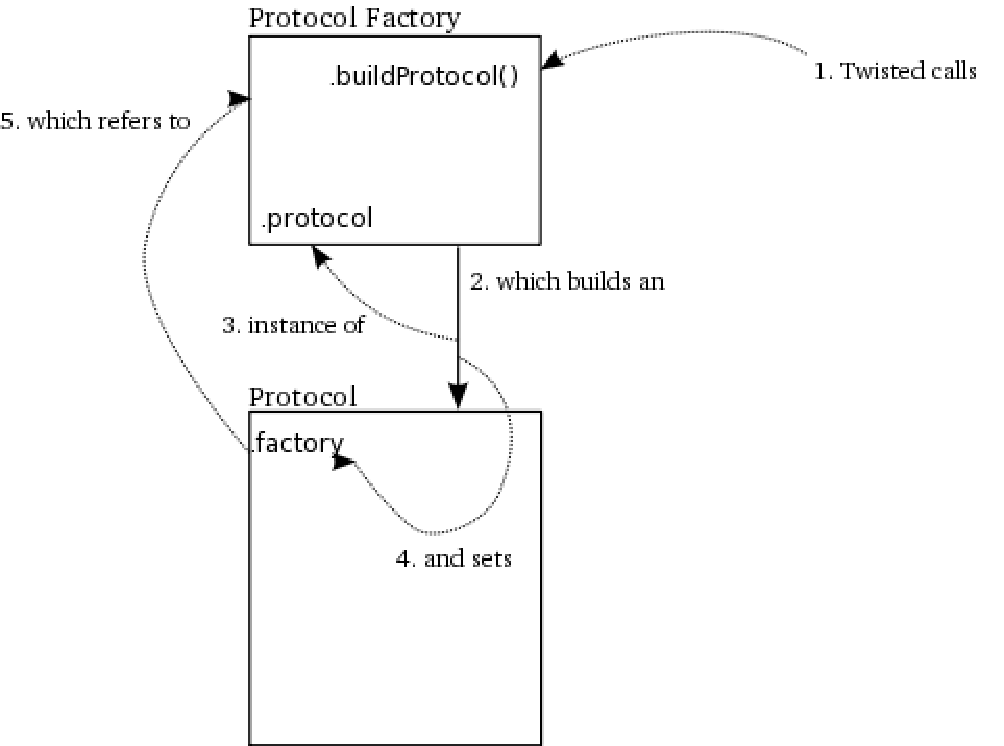
\includegraphics[width=0.7\textwidth]{images/protocols-1.pdf}
    \caption{Рождение Protocol'а\label{fig:protocols-1}}
\end{center}
\end{figure}


%As we mentioned above, the factory attribute on Protocol objects allows Protocols created with the same Factory to share state. And since Factories are created by “user code”, that same attribute allows Protocol objects to communicate results back to the code that initiated the request in the first place, as we will see in Part 6.

Как мы упомянули выше, атрибут factory в объектах 
типа Protocol позволяют протоколам, созданным одним 
и тем же объектом типа Factory, разделять состояние. И 
поскольку фабрики создаются пользовательским кодом, 
одинаковый атрибут позволяет объектам типа Protocol 
передавать результаты обратно в код, который задал запрос,  
как мы увидим в главе 6. 

%Note that while the factory attribute on Protocols refers to an instance of a Protocol Factory, the protocol attribute on the Factory refers to the class of the Protocol. In general, a single Factory might create many Protocol instances.

Заметьте, что в то время как атрибут factory в 
Protocol'ах ссылается на экземпляр Protocol Factory, 
атрибут protocol в Factory ссылается на класс Protocol. 
В общем случае, один объект Factory может создать 
много экземпляров Protocol.

%The second stage of Protocol construction connects a Protocol with a Transport, using the makeConnection method. We don’t have to implement this method ourselves since the Twisted base class provides a default implementation. By default, makeConnection stores a reference to the Transport on the transport attribute and sets the connected attribute to a True value, as depicted in Figure 9:

Вторая стадия создания Protocol соединяет Protocol с 
Transport, используя метод makeConnection. Мы не должны 
реализовывать этот метод сами, поскольку базовый класс в 
Twisted предоставляет реализацию по умолчанию. По умолчанию, 
makeConnection сохраняет ссылку на Transport в атрибуте 
transport и устанавливает атрибут connected в значение Truе, 
как это изображено на рисунке \ref{fig:protocols-2}:

% fig9
\begin{figure}[h]
\begin{center}
    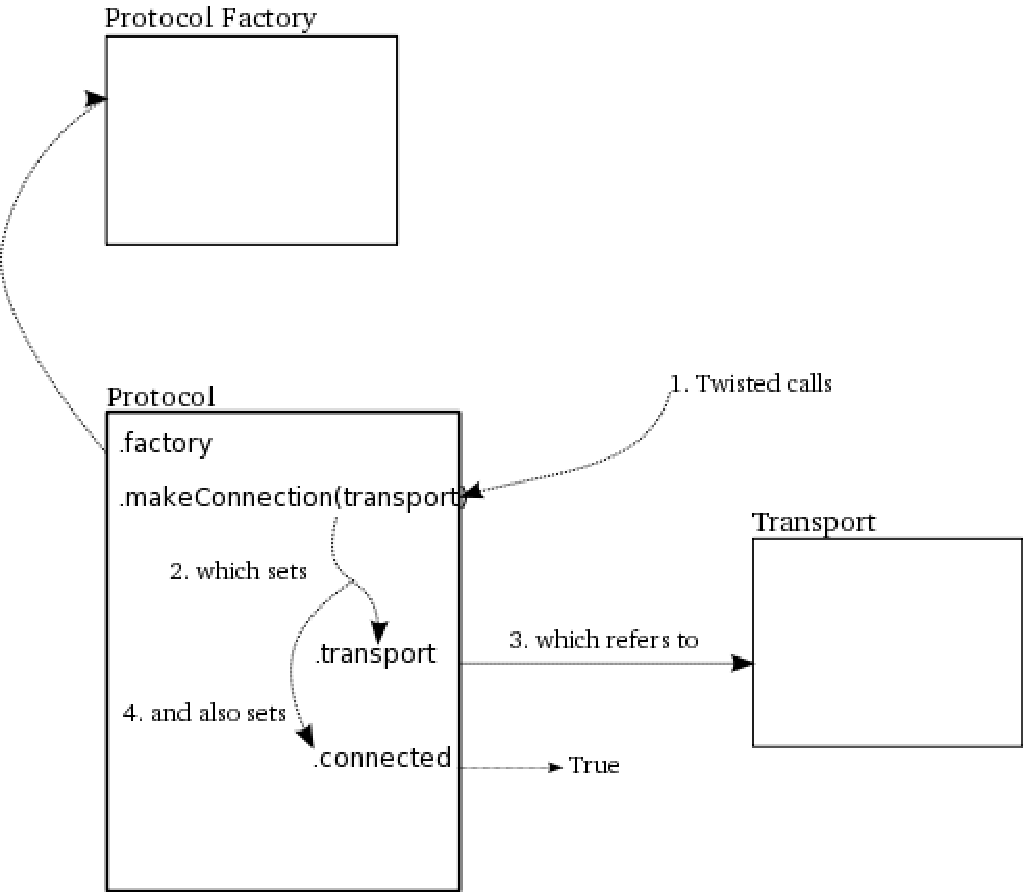
\includegraphics[width=0.7\textwidth]{images/protocols-2.pdf}
    \caption{Ссылка из Protocol в Transport\label{fig:protocols-2}}
\end{center}
\end{figure}


%Once initialized in this way, the Protocol can start performing its real job — translating a lower-level stream of data into a higher-level stream of protocol messages (and vice-versa for 2-way connections). The key method for processing incoming data is dataReceived, which our client implements like this:

Однажды проинициализировав таким образом, Protocol 
может начать выполнение своей реальной работы - 
передачу низкоуровневого потока данных в высокоуровневый 
поток протокольных сообщений (и, наоборот, для двунаправленных соединений). 
Ключевой метод для обработки приходящих данных - dataReceived, 
который наш клиент реализовывает следующим образом:

\begin{scriptsize}\begin{verbatim}
def dataReceived(self, data):
    self.poem += data
    msg = 'Task %d: got %d bytes of poetry from %s'
    print  msg % (self.task_num, len(data), self.transport.getHost())
\end{verbatim}\end{scriptsize}

%Each time dataReceived is called we get a new sequence of bytes (data) in the form of a string. As always with asynchronous I/O, we don’t know how much data we are going to get so we have to buffer it until we receive a complete protocol message. In our case, the poem isn’t finished until the connection is closed, so we just keep adding the bytes to our .poem attribute.

Каждый раз при вызове dataReceived мы получаем новую 
последовательность байт (данных) в форме строки. 
Как всегда с асинхронным вводом-выводом, мы не знаем как много данных 
мы получим, так что мы должны буферизовать их, до тех пор пока мы 
не получим завершенное протокольное сообщение. В нашем случае, поэма не 
завершается до тех пор, пока не закроется соединение, поэтому мы 
добавляем байты в наш атрибут poem.


%Note we are using the getHost method on our Transport to identify which server the data is coming from. We are only doing this to be consistent with earlier clients. Otherwise our code wouldn’t need to use the Transport explicitly at all, since we never send any data to the servers.

Заметьте, что мы используем метод 
\href{http://twistedmatrix.com/trac/browser/tags/releases/twisted-8.2.0/twisted/internet/interfaces.py#L1341}{getHost} 
нашего Transport'а для идентификации того, какой с какого сервера пришли данные. 
Мы делаем это только для согласованности с более ранними клиентами. 
Иначе, нашему коду не нужно было бы использовать Transport явно, поскольку 
мы никогда не отправляем данные серверу. 


%Let’s take a quick look at what’s going on when the dataReceived method is called. In the same directory as our 2.0 client, there is another client called twisted-client-2/get-poetry-stack.py. This is just like the 2.0 client except the dataReceived method has been changed like this:

Давайте посмотрим на то, что происходит, когда вызвается метод dataReceived. 
В той же директории, где находится наш клиент 2.0, есть еще один клиент в файле 
twisted-client-2/get-poetry-stack.py. Это тоже самое, что и клиент 2.0, за 
исключением того, что метод dataReceived изменен следующим образом: 

\begin{scriptsize}\begin{verbatim}
def dataReceived(self, data):
    traceback.print_stack()
    os._exit(0)
\end{verbatim}\end{scriptsize}

%With this change the program will print a stack trace and then quit the first time it receives some data. You could run this version like so:
С этим изменением программа будет печатать stack trace и затем 
завершится сразу после получения некоторых данных. Вы можете 
запустить эту версию следующим образом:

\begin{scriptsize}\begin{verbatim}
python twisted-client-2/get-poetry-stack.py 10000
\end{verbatim}\end{scriptsize}

%And you will get a stack trace like this:
И вы получите следующий stack trace:

\begin{scriptsize}\begin{verbatim}
File "twisted-client-2/get-poetry-stack.py", line 125, in
    poetry_main()

... # I removed a bunch of lines here

File ".../twisted/internet/tcp.py", line 463, in doRead  # Note the doRead callback
    return self.protocol.dataReceived(data)
File "twisted-client-2/get-poetry-stack.py", line 58, in dataReceived
    traceback.print_stack()
\end{verbatim}\end{scriptsize}

%There’s the doRead callback we used in client 1.0! As we noted before, Twisted builds new abstractions by using the old ones, not by replacing them. So there is still an IReadDescriptor implementation hard at work, it’s just implemented by Twisted instead of our code. If you are curious, Twisted’s implementation is in twisted.internet.tcp. If you follow the code, you’ll find that the same object implements IWriteDescriptor and ITransport too. So the IReadDescriptor is actually the Transport object in disguise. We can visualize a dataReceived callback with Figure 10:

В выводе мы видим doRead callback, который мы использовали в клиенте 1.0! 
Как было замечено ранее, Twisted создает новые абстракции, используя 
старые, но не заменяя их. То есть здесь в работе все еще реализация IReadDescriptor, 
но она реализована внутри Twisted, а не в нашем коде. Если вы любопытны, то 
реализация находится в twisted.internet.tcp. Если вы посмотрите в код, то найдете 
похожий объект, реализующий IWriteDescriptor и ITransport. Так что IReadDescriptor - 
это в действительности замаскированный объект типа Transport. Мы можем визуализировать 
dataReceived callback как на рисунке \ref{fig:reactor-data-received}:

% fig10
\begin{figure}[h]
\begin{center}
    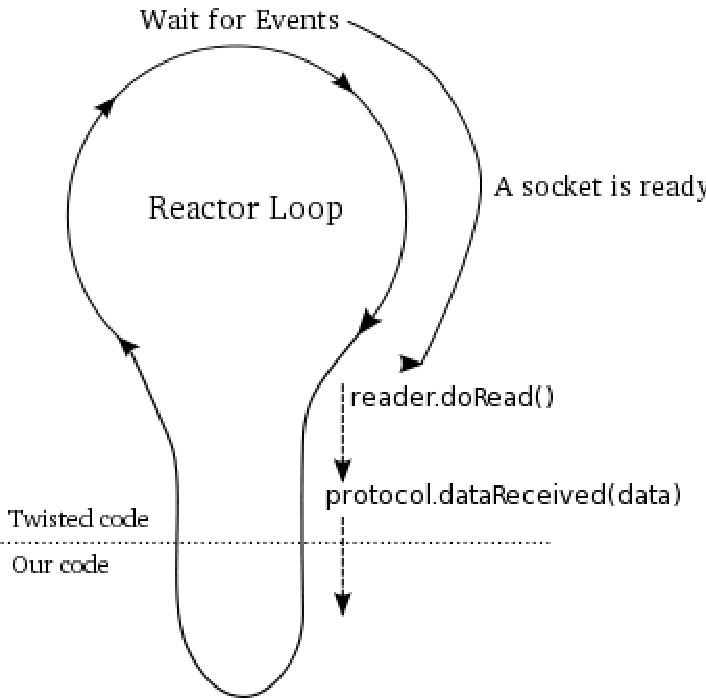
\includegraphics[width=0.5\textwidth]{images/reactor-data-received.pdf}
    \caption{dataReceived callback\label{fig:reactor-data-received}}
\end{center}
\end{figure}

%Once a poem has finished downloading, the PoetryProtocol object notifies its PoetryClientFactory:
Сразу же, когда поэма скачалась, объект PoetryProtocol сообщает 
об этом PoetryClientFactory:

\begin{scriptsize}\begin{verbatim}
def connectionLost(self, reason):
    self.poemReceived(self.poem)

def poemReceived(self, poem):
    self.factory.poem_finished(self.task_num, poem)
\end{verbatim}\end{scriptsize}

%The connectionLost callback is invoked when the transport’s connection is closed. The reason argument is a twisted.python.failure.Failure object with additional information on whether the connection was closed cleanly or due to an error. Our client just ignores this value and assumes we received the entire poem.

callback connectionLost вызывается при закрытии транспортного соединения. 
Аргумент reason - это объект типа 
\href{http://twistedmatrix.com/trac/browser/tags/releases/twisted-8.2.0/twisted/python/failure.py}{twisted.python.failure.Failure} 
с дополнительной информацией о том закрылось ли соединение без ошибок 
или из-за ошибок. Наш клиент просто игнорирует это значение и предполагает, 
что мы получили поэму полностью.

%The factory shuts down the reactor after all the poems are done. Once again we assume the only thing our program is doing is downloading poems, which makes PoetryClientFactory objects less reusable. We’ll fix that in the next Part, but notice how the poem_finished callback keeps track of the number of poems left to go:

factory останавливает reactor после того, как все поэмы скачались. 
И снова мы предполагаем, что единственное, что наша программа 
делает - скачивает поэмы, что делает объекты типа PoetryClientFactory 
менее переиспользуемыми. Мы исправим это в следующей главе, но заметьте 
то, как poem\_finished callback сохраняет количество оставшихся поэм:

\begin{scriptsize}\begin{verbatim}
...
    self.poetry_count -= 1

    if self.poetry_count == 0:
        ...
\end{verbatim}\end{scriptsize}

%If we were writing a multi-threaded program where each poem was downloaded in a separate thread we would need to protect this section of code with a lock in case two or more threads invoked poem_finished at the same time. Otherwise we might end up shutting down the reactor twice (and getting a traceback for our troubles). But with a reactive system we needn’t bother. The reactor can only make one callback at a time, so this problem just can’t happen.

Если бы мы писали многотредовую программу, где каждая 
поэма скачивается в отдельном потоке, нам бы 
понадобилось защищать участок программы выше с помощью 
lock'а в случае двух или более потоков, вызывающих 
poem\_finished в одно и то же время. Иначе, мы могли бы 
завершить reactor дважды (и получить исключение). Но с 
реактивной системой нам не нужно об этом заботиться: reactor 
может вызывать только один callback за раз, так что такая  
проблема не может произойти.

%Our new client also handles a failure to connect with more grace than the 1.0 client. Here’s the callback on the PoetryClientFactory class which does the job:

Наш новый клиент управляет ошибкой соединения 
изящнее, чем в клиент 1.0. Следующий callback в 
классе PoetryClientFactory делает это:

\begin{scriptsize}\begin{verbatim}
def clientConnectionFailed(self, connector, reason):
    print 'Failed to connect to:', connector.getDestination()
    self.poem_finished()
\end{verbatim}\end{scriptsize}

%Note the callback is on the factory, not on the protocol. Since a protocol is only created after a connection is made, the factory gets the news when a connection cannot be established.

Заметьте, что callback находится в Factory, а не в Protocol. 
Поскольку Protocol создается только после создания соединения, 
а Factory получает новости о том, что соединение не установилось.


\subsection{Упрощение клиента}

%Although our new client is pretty simple already, we can make it simpler if we dispense with the task numbers. The client should really be about the poetry, after all. There is a simplified 2.1 version in twisted-client-2/get-poetry-simple.py.

Хотя наш клиент уже достоточно прост, мы можем еще больше его 
упростить, если обойдемся без номеров задач. Клиент ведь реально 
о поэзии в конце концов. Упрощенная версия клиента 2.1 находится в   
\href{http://github.com/jdavisp3/twisted-intro/blob/master/twisted-client-2/get-poetry-simple.py}{twisted-client-2/get-poetry-simple.py}.

\subsection{Резюме}

%Client 2.0 uses Twisted abstractions that should be familiar to any Twisted hacker. And if all we wanted was a command-line client that printed out some poetry and then quit, we could even stop here and call our program done. But if we wanted some re-usable code, some code that we could embed in a larger program that needs to download some poetry but also do other things, then we still have some work to do. In Part 6 we’ll take a first stab at it.

Клиент 2.0 использует Twisted абстрации, которые 
знакомы любому Twisted хакеру. И если все, что мы хотели - 
это клиент, запускающийся из командной строки, печатающий 
некоторую поэзию и после - завершающийся, то мы могли бы здесь остановится и 
сказать, что наша программа сделана. Но если вы хотите некоторый 
переиспользуемый код, который вы могли 
бы встроить в большую программу, которой надо было 
скачать немного поэзии и сделать также другие вещи, то у нас все 
еще есть над чем работать. В главе 6 мы сделаем первый удар в эту сторону.

\subsection{Упражнения}

\begin{enumerate}
%   1. Use callLater to make the client timeout if a poem hasn’t finished after a given interval. Use the loseConnection method on the transport to close the connection on a timeout, and don’t forget to cancel the timeout if the poem finishes on time.
\item Используйте callLater для того, чтобы сделать timeout для клиента, 
если поэма не скачалась после заданного интервала времени. 
Используйте метод loseConnection класса Transport  для того, чтобы закрыть соединение 
при возникновлении timeout'а, и не забудьте сбросить timeout, если 
поэма скачалась во время. 
%   2. Use the stacktrace method to analyze the callback sequence that occurs when connectionLost is invoked.
\item Используйте метод stacktrace для анализа последовательности 
callback'ов, которые вызываются в момент вызова connectionLost.
\end{enumerate}

